\chapter{Context}
\section{P\^{o}le Universitaire Fran\c{c}ais}
The P\^{o}le Universitaire Fran\c{c}ais (PUF) was created by the intergovernmental agreement of VietNam and France in October 2004. With ambition is building a linking program between the universities in VietNam and the advanced programs of universities in France. There are two PUF's center in VietNam: P\^{o}le Universitaire Fran\c{c}ais de l'Universite National\'{e} du Vietnam - Ha Noi located in Ha Noi capital (PUF-Ha Noi) and P\^{o}le Universitaire Fran\c{c}ais de l'Universite National\'{e} du Vietnam - Ho Chi Minh Ville located in Ho Chi Minh city (PUF-HCM).
\iffalse
\subsection{PUF-Ha Noi}
PUF-Ha Noi is regarded as a nursery for the linking program, it support on administrative procedure and logistics for the early year of program. Besides, PUF-Ha Noi also implement the training program regularly about Master 2 provided by universities and academies in France. About administration, PUF-HN directly under Institut Francophone International (IFI), which was created by VietNam National University at HaNoi in 2012.
\fi
\subsection*{PUF-HCM}
PUF-HCM\footnote{http://pufhcm.edu.vn} is a department of VietNam National Univeristy at Ho Chi Minh city. From the first year of operations, PUF-HCM launched the quality training programs from France in VietNam. With target, bring the programs which designed and evaluated by the international standards for Vietnamese student. PUF-HCM always strive in our training work.\\
So far, PUF-HCM have five linking programs with the universities in France, and the programs are organized into the subjects: Commerce, Economic, Management and Informatics. In detail:
\begin{itemize}
\item Bachelor and Master of Economics : linking program with University of Toulouse 1 Captiole
\item Bachelor and Master of Informatics: linking program with University of Bordeaux and University of Paris 6.
\end{itemize}
The courses in PUF-HCM are provided in French, English and Vietnamese by both Vietnamese and French professors. The highlight of the programs are inspection and diploma was done by the French universities.
\section{Laboratoire Bordelais de Recherche en Informatique}
The Laboratoire Bordelais de Recherche en Informatique (LaBRI)\footnote{http://www.labri.fr} is a research unit associated with the CNRS (URM 5800), the University of Bordeaux and the Bordeaux INP. Since 2002, it has been the partner of Inria. It has significantly increased in staff numbers over recent years. In March 2015, it had a total of 320 members including 113 teaching/research staff (University of Bordeaux and Bordeaux INP), 37 research staff (CNRS and Inria), 22 administrative and technical (University of Bordeaux, Bordeaux INP, CNRS and Inria) and more than 140 doctoral students and post-docs. The LaBRI's missions are: research (pure and applied), technology application and transfer and training.\\
Today the members of the laboratory are grouped in six teams, each one combining basic research, applied research and technology transfer:
\begin{itemize}
\item Combinatorics and Algorithmic
\item Image and Sound
\item Formal Methods
\item Models and Algorithms for Bio-informatics and Data Visualisation
\item Programming, Networks and Systems
\item Supports and Algorithms for High Performance Numerical Applications
\end{itemize} 
Within these team, research activities are conducted in partnership with Inria. Besides that, LaBRI also collaborate with many other laboratories and companies on French, European and the international.
\newpage
\section{The Internship}
The internship is intended to be a duration to apply the knowledge to the real environment. It shows the ability synthesis, evaluation and self-research of student. Besides, the student may study the experience from the real working environment. My internship is done under the guidance of Mrs Marie BEURTON-AIMAR in a period of six months at LaBRI laboratory.\\[0.2cm]
As a part of collaboration between LaBRI and INRA Rennes, the project is working on the agriculture field. The goals of the project is tracking, collecting and classifying the insects based on the morphometry of them, specific beetle. Biologists from Rennes have collected a set of 293 beetles and produced a series of images for the different parts of beetle such as head, body, right mandible, left mandible and pronotum (see in figure \ref{fig:figure_11}). The main request from the biologist team is: \textit{"How to produce automatically landmarks on each image that could be equivalent to manual landmarks (landmarks set by hand)?"}.
\begin{figure}[h!]
\centering
\subfloat[Body part of beetle]
{\label{fig:example_111}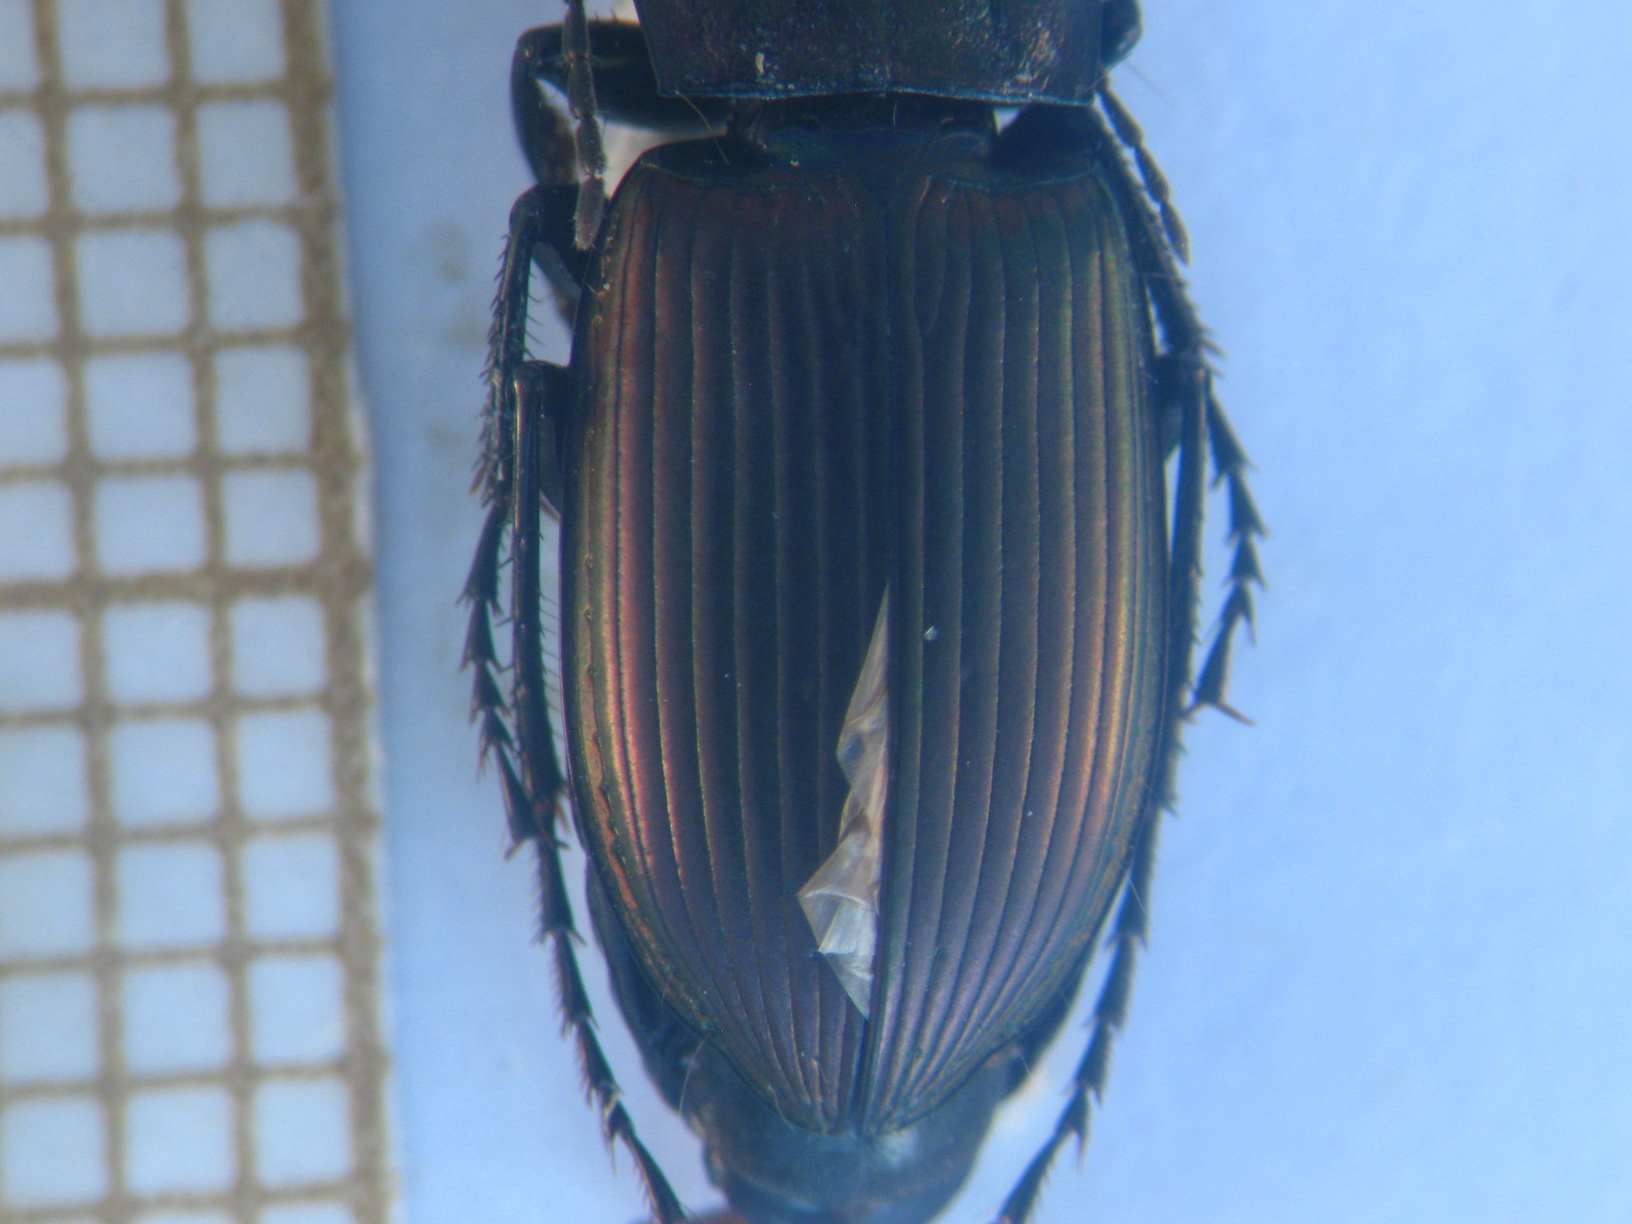
\includegraphics[width=0.45\textwidth]{./images/input1}}~~
\subfloat[Pronotum part of beetle]
{\label{fig:example_112}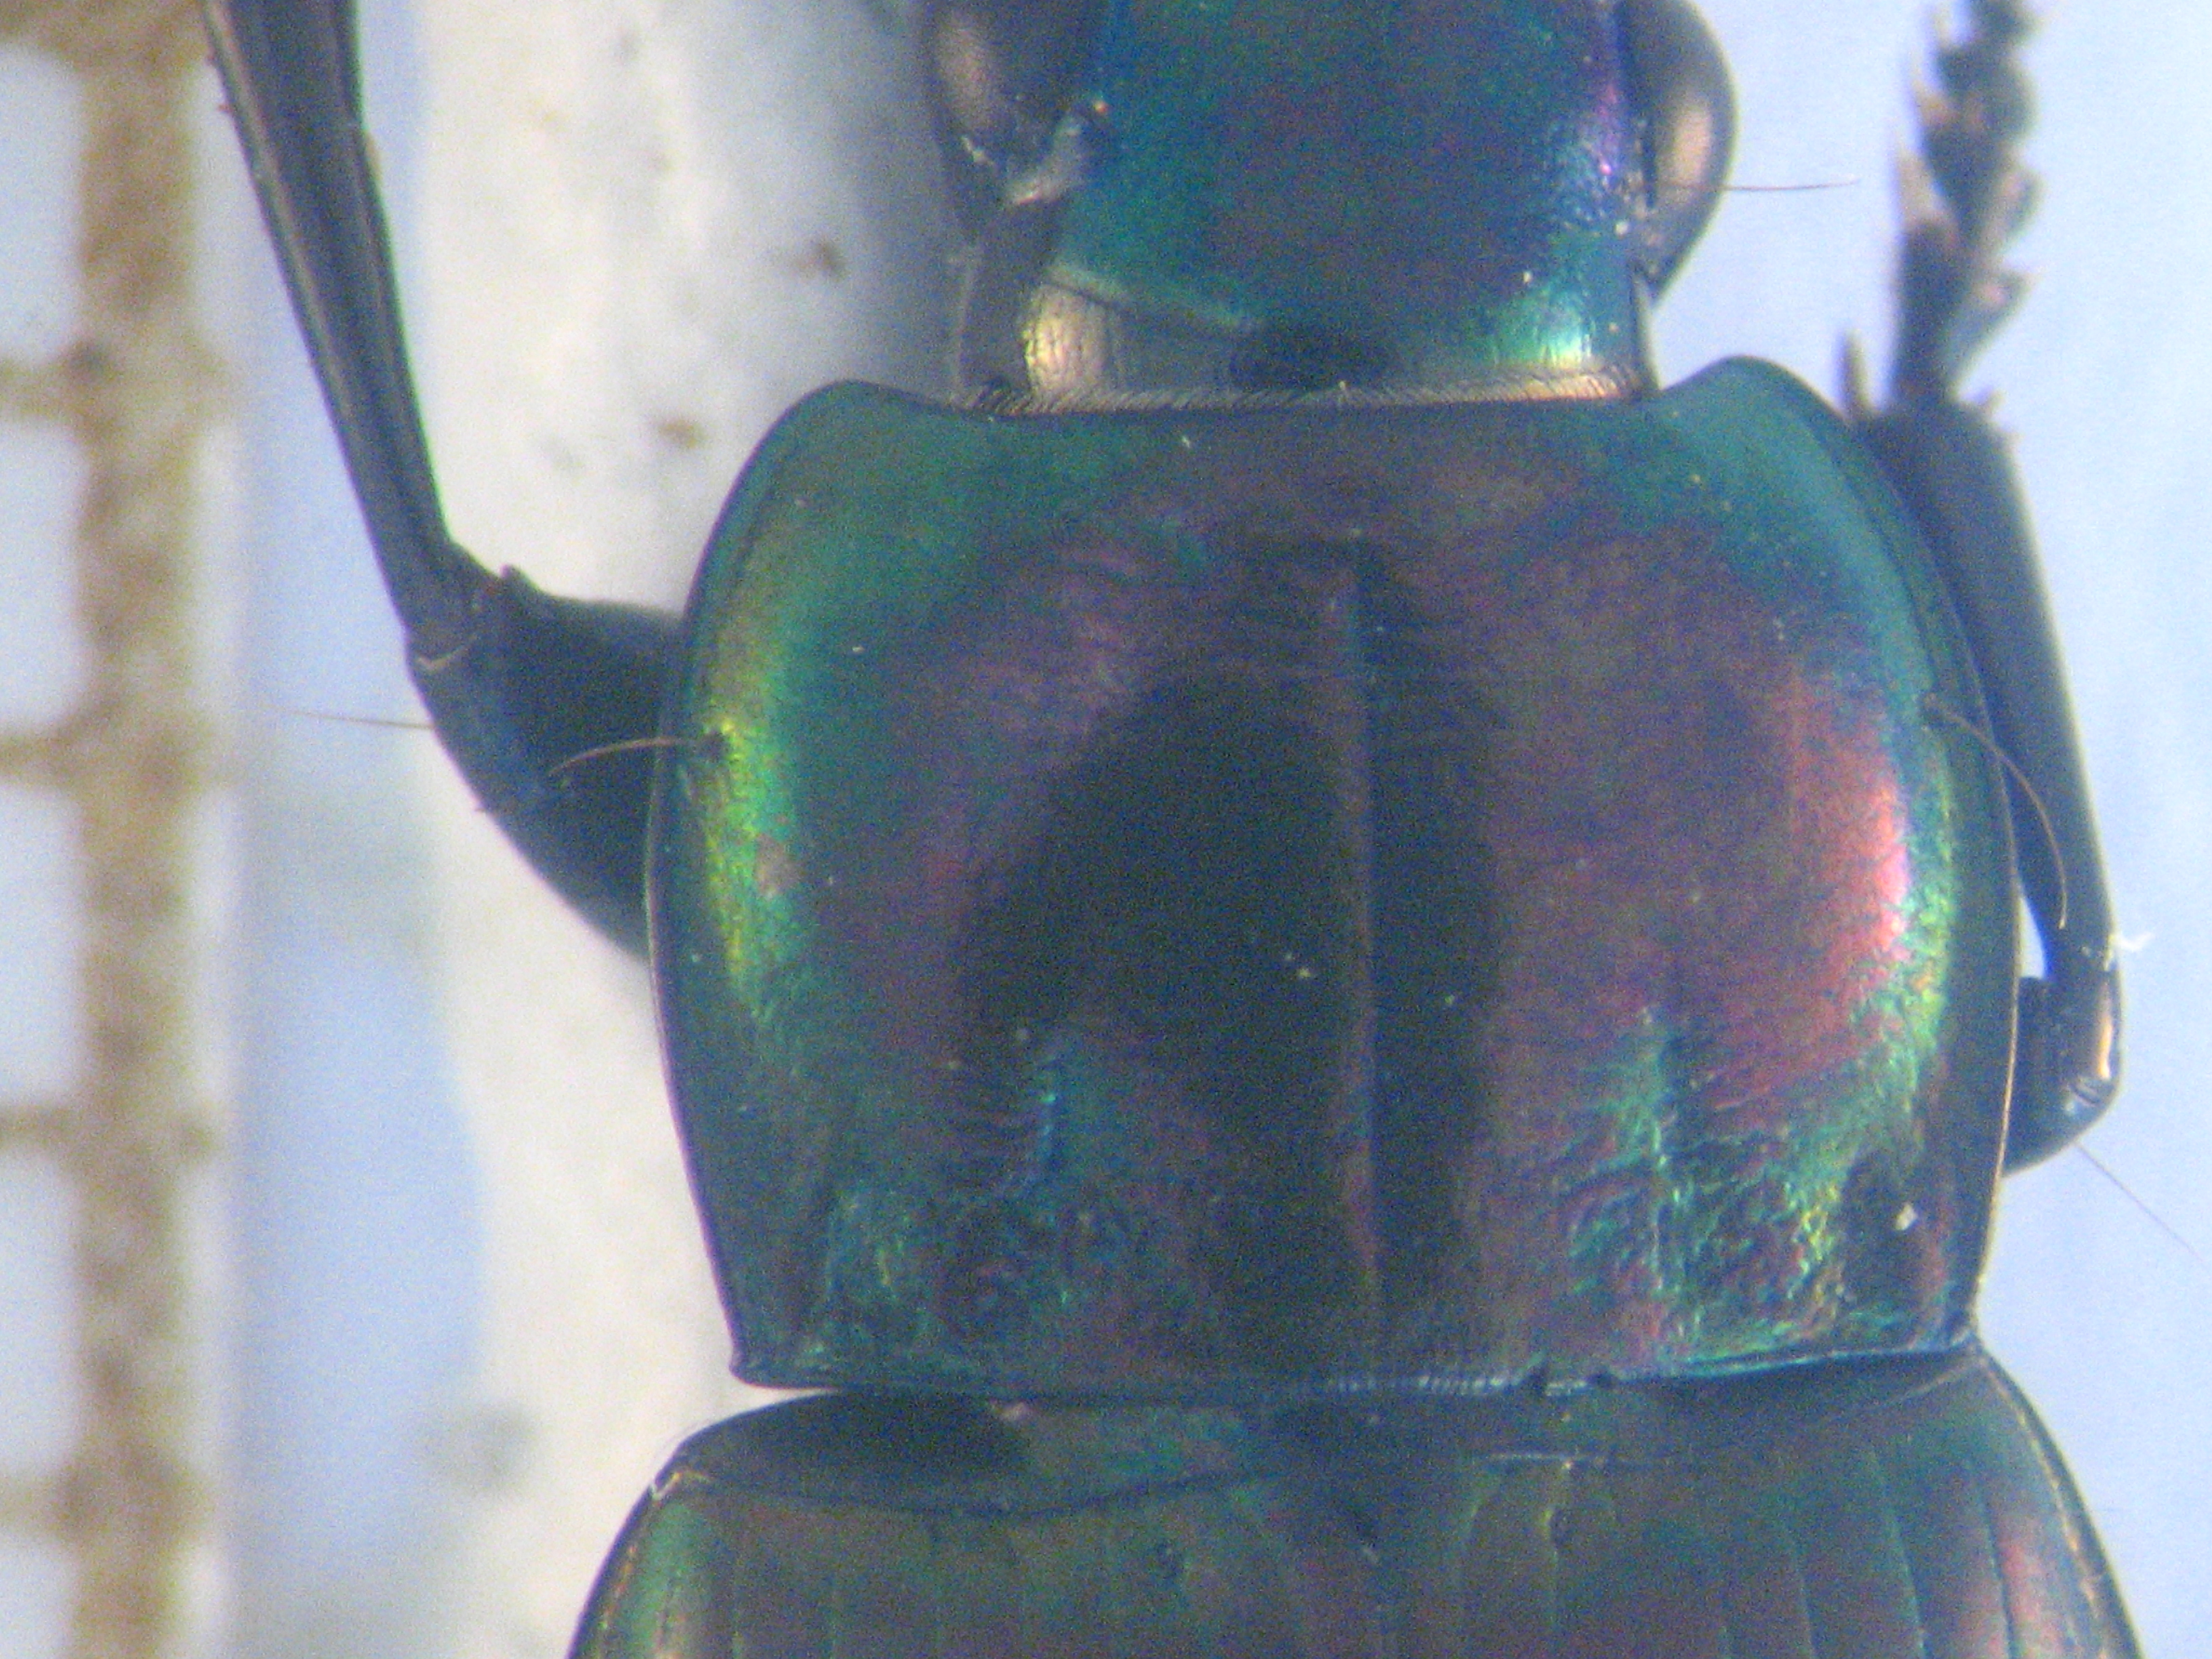
\includegraphics[width=0.45\textwidth]{./images/prono006}}\\
\subfloat[Right mandible of beetle]{\label{fig:example_113}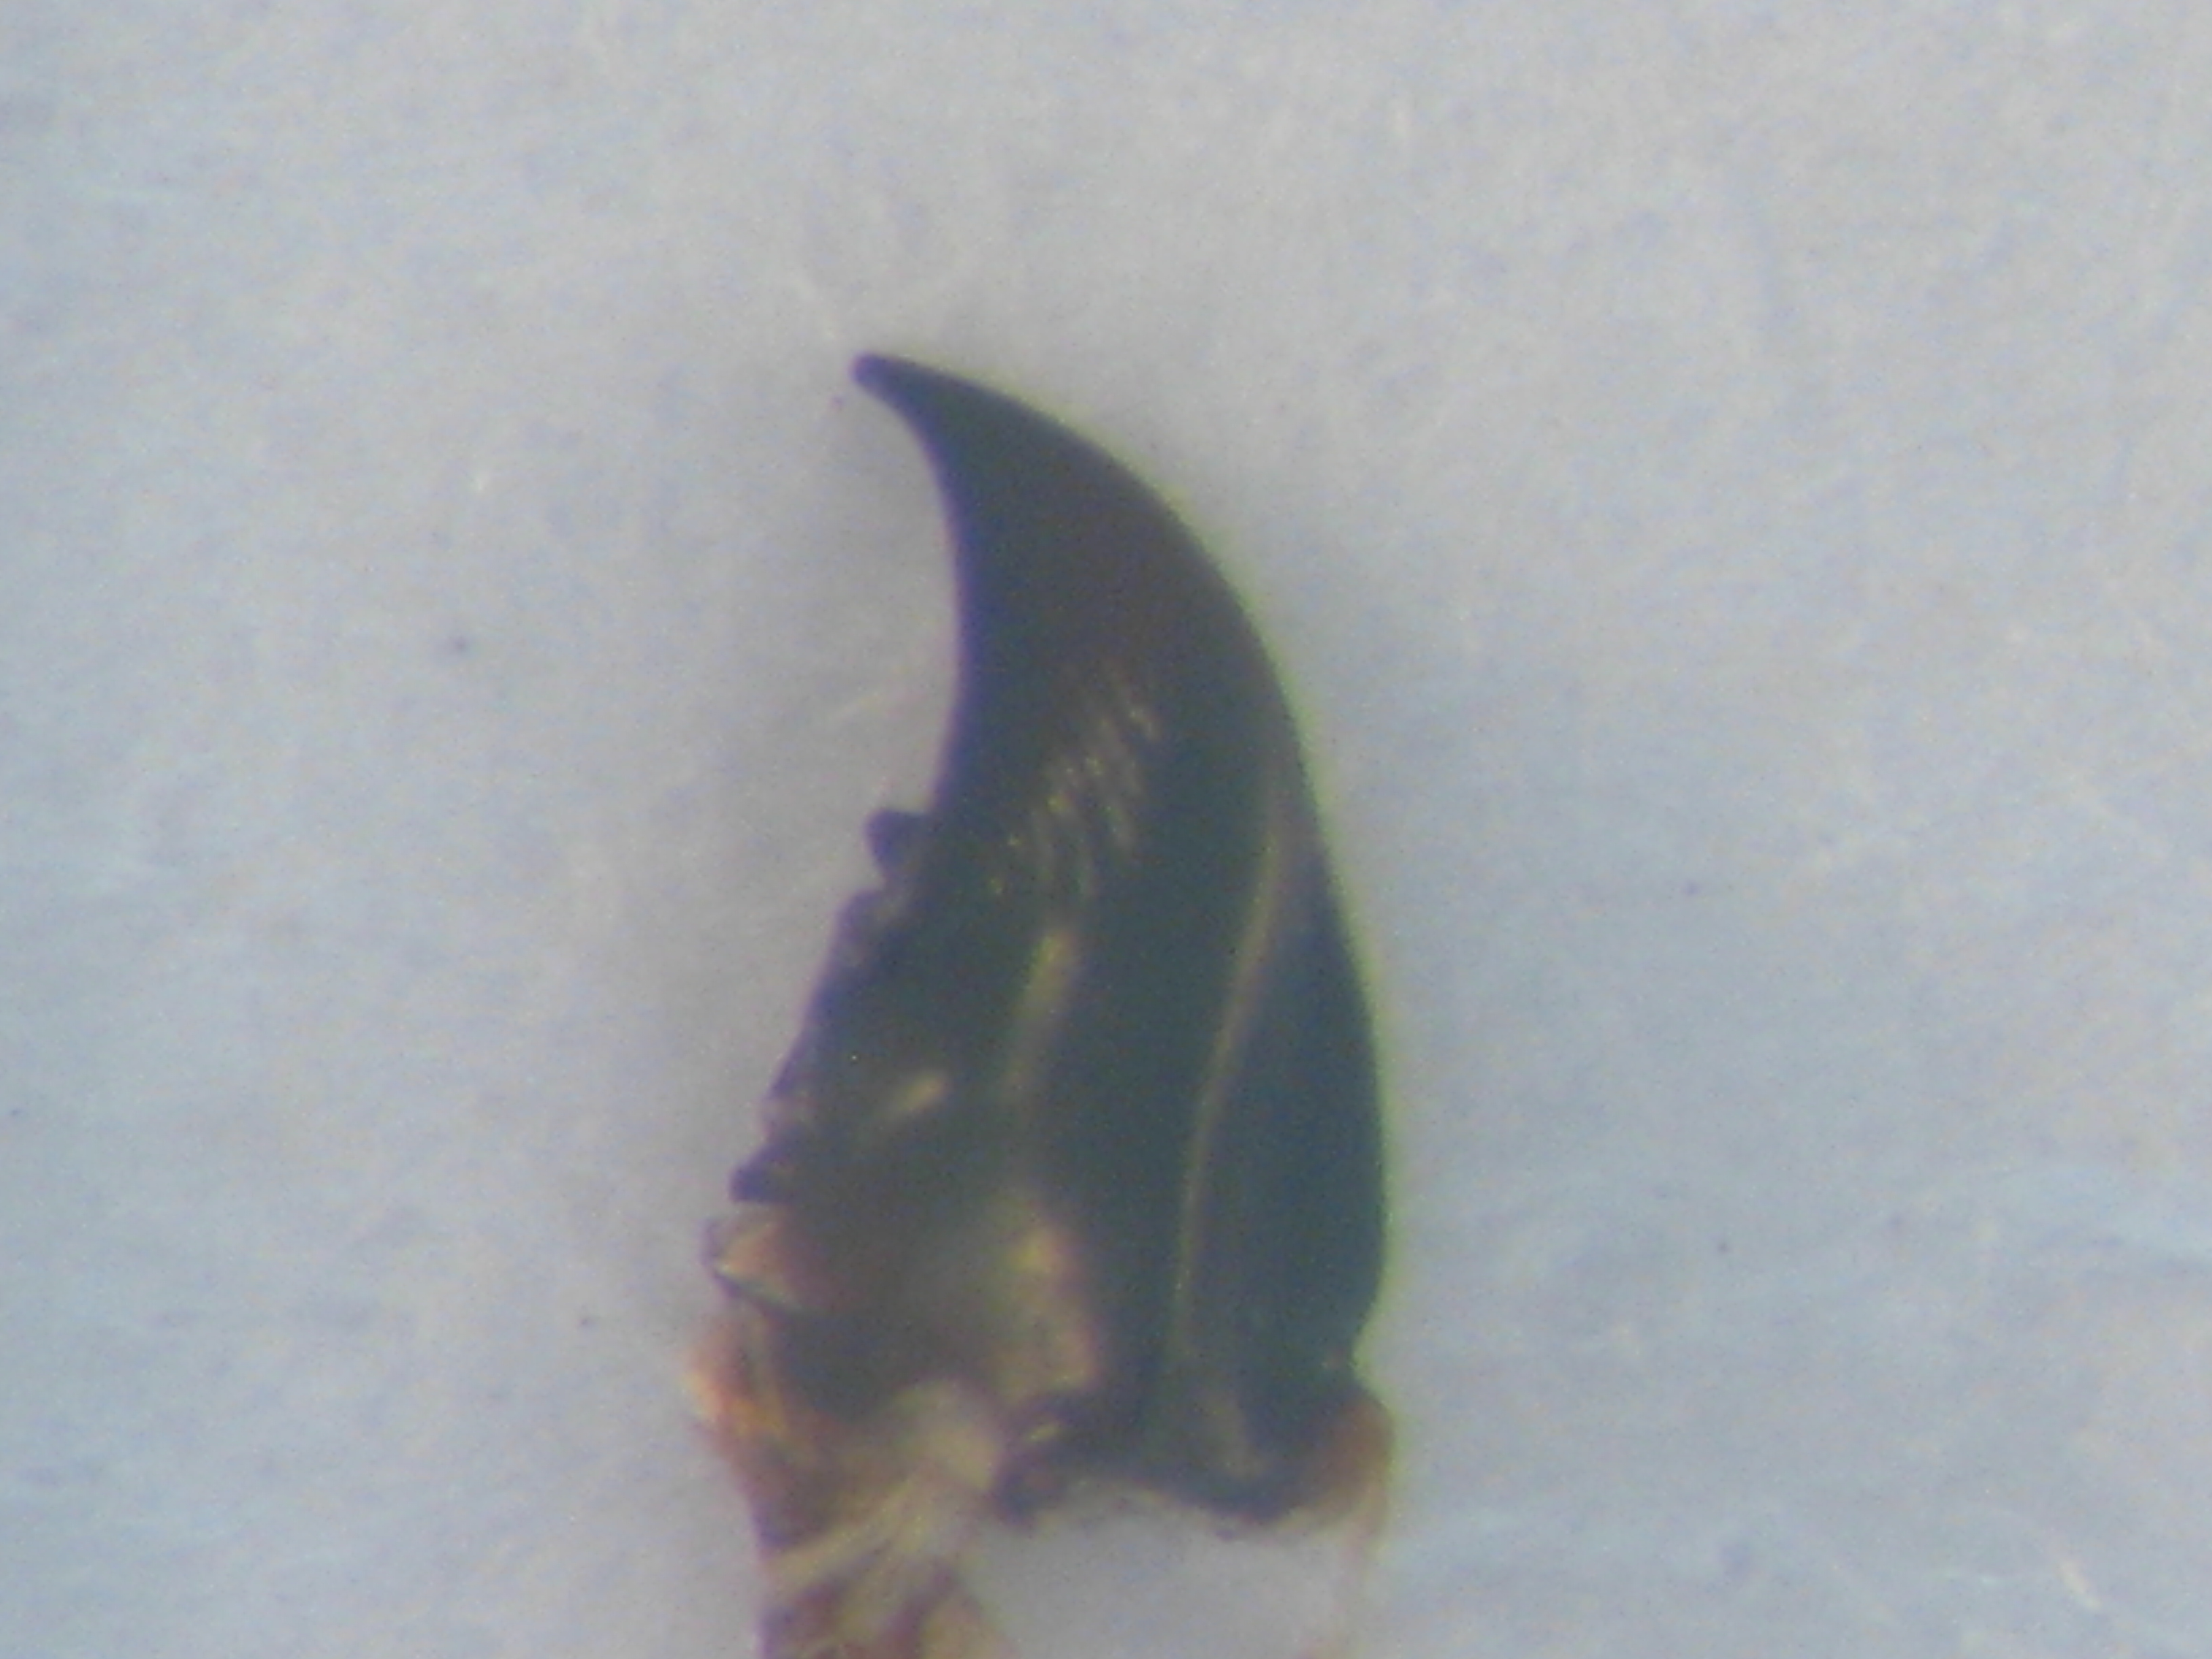
\includegraphics[width=0.45\textwidth]{./images/md32}}~~
\subfloat[Left mandible of beetle]
{\label{fig:example_114}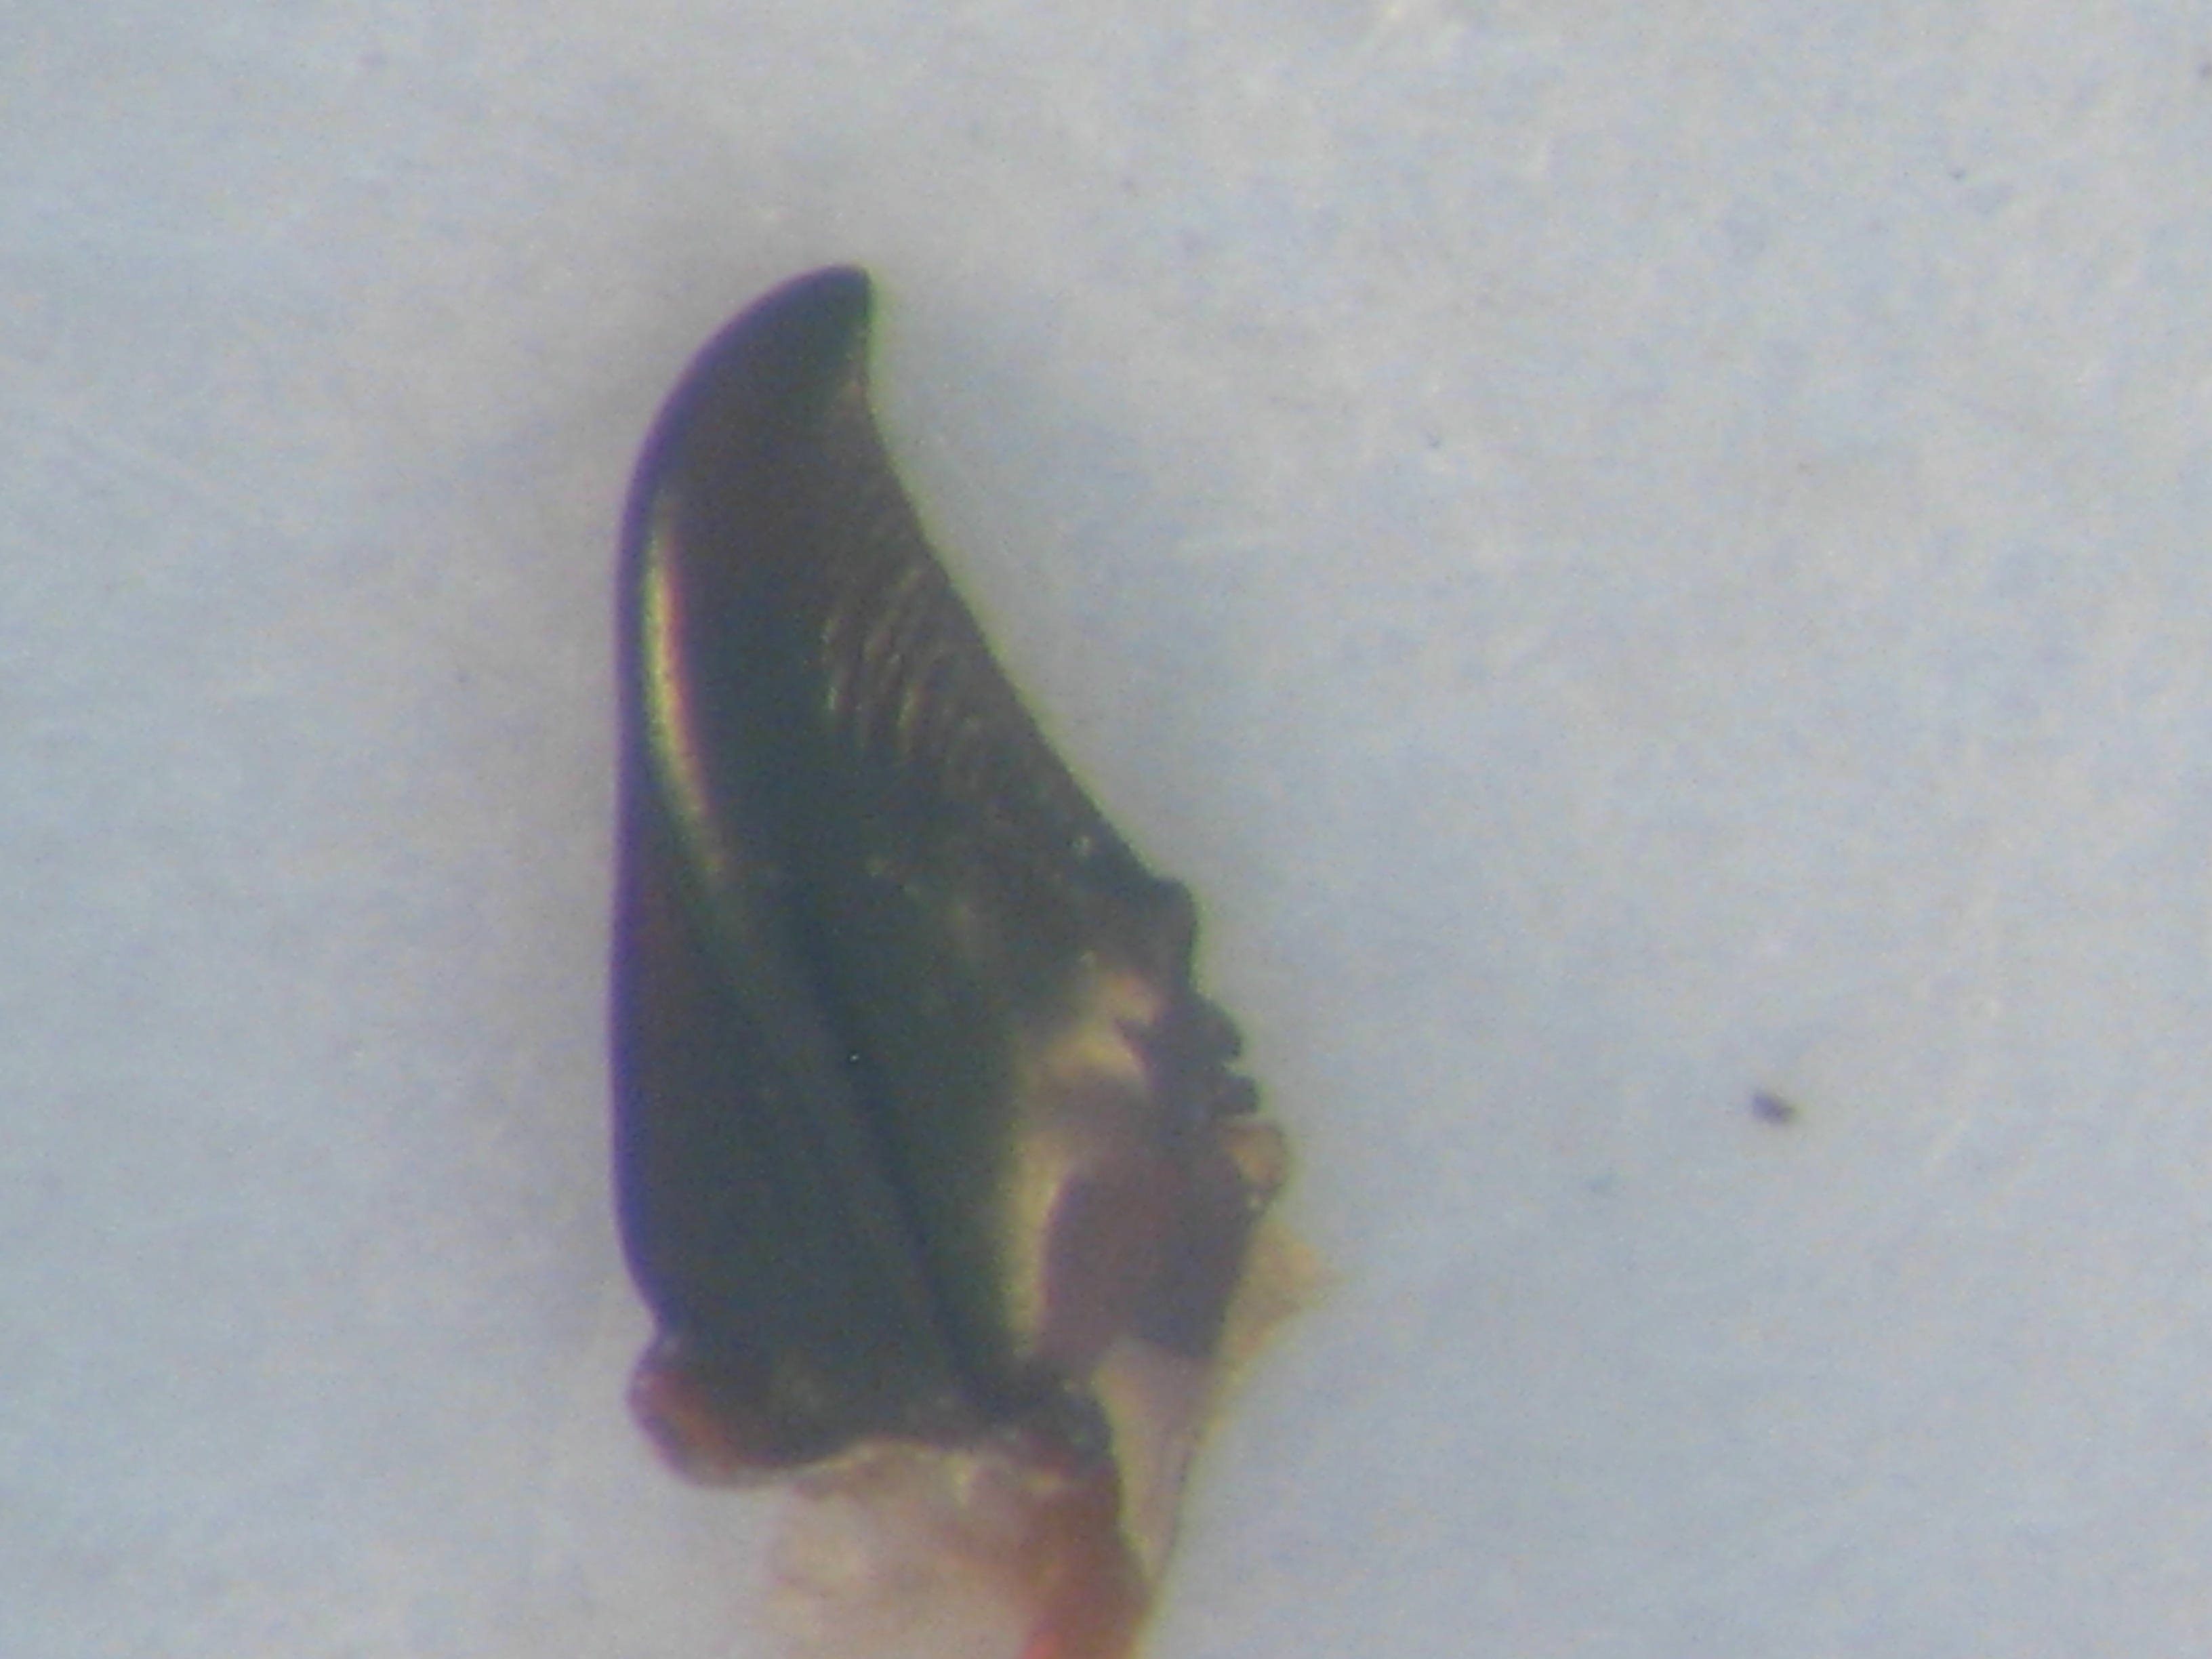
\includegraphics[width=0.45\textwidth]{./images/mg29}}\\
\subfloat[Head of beetle]
{\label{fig:example_115}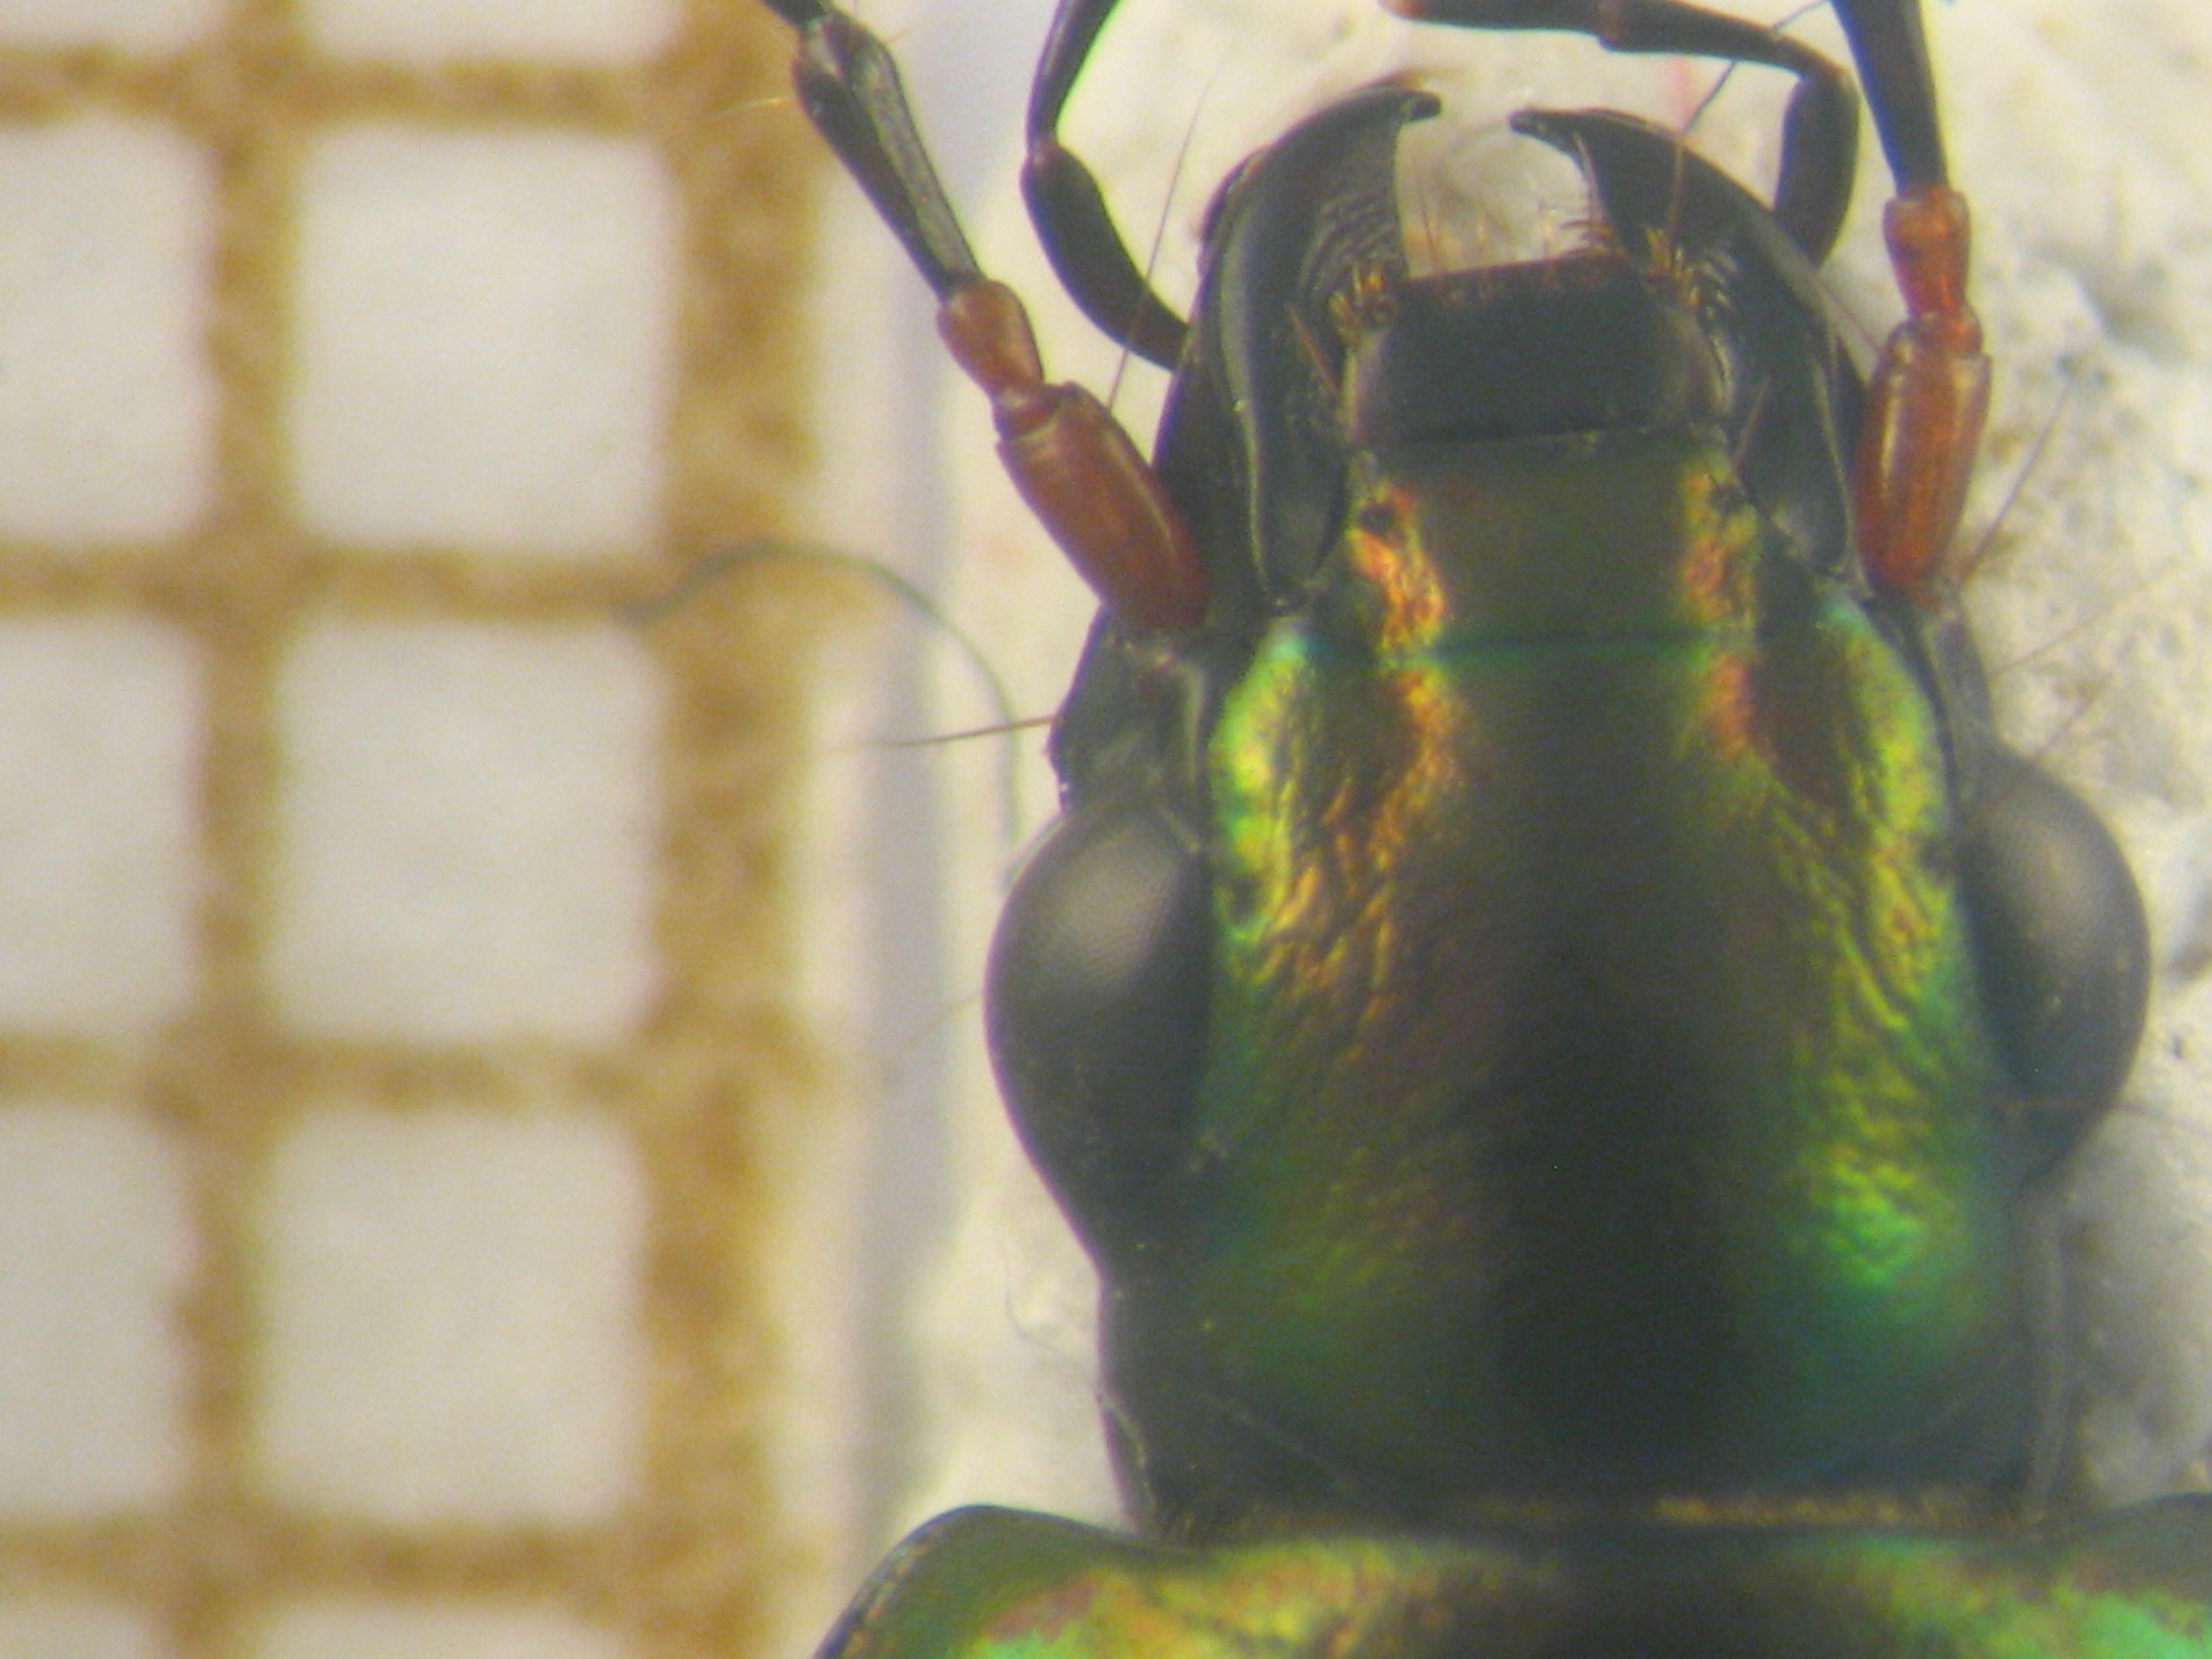
\includegraphics[width=0.45\textwidth]{./images/tete111}}
\caption{The parts of beetle}
\label{fig:figure_11}
\end{figure}~\\[0.2cm]
\textit{``Morphometric landmarks are points that can be defined in all specimens  and located precisely"}\cite{palaniswamy2010automatic}. They are widely used in many biological and medical applications. Presently, the landmarks are mainly extracted manually. Doing that automatically remains a challenge.\\[0.2cm]
The objectives of this internship is implementing a method to automatic extract landmarks. The method based on the article: \textbf{``Automatic identification of landmarks in digital images"}, which proposed by Palaniswamy\cite{palaniswamy2010automatic}. Besides, an evaluation about accuracy of method is done based on the comparing between the estimated landmarks and the manual landmarks which have been set by biologists.